In \cite{bib_01}, the solution of dynamic object type identification is proposed to implement automatically with the wavelet-fractal-correlation algorithm for processing samples of measurements of the coordinates for the elevation angle, azimuth and range of the detected DO optoelectron device (OED) in the final sliding time interval with a priori uncertainty about the actual current phono-target situation in the device control zone.
During the movement, the DO can maneuver and be observed by OED from different angles.
As a result, the intensity of the DO optical radiation in the direction of the OED will represent a non-stationary space-time random process with an unknown probability distribution law.
In samples of measurements of DO coordinates, "outliers" and fluctuations can appear.
In Fig.~\ref{fig:fig_1_option_1}, Fig.~\ref{fig:fig_1_option_2}, Fig.~\ref{fig:fig_1_option_3} shows such samples obtained by real DO on various trajectories of their movement in the zone of control of OED (the abscissa axis in the figures shows the number of phono-target frames formed by the OED, that is, the sample sizes, and the ordinate axis is kilometers and degrees).

Obviously, this will determine the different significance of individual measurements and the effect on the result reliability producing by the recognition algorithm of the detected DO type.
It is not possible to reduce the influence through the implementation of the adaptation principle due to a priori uncertainty regarding the nonstationarity of the current phono-target situation in the zone of OED control.

Because of this, there arises an objective necessity to build an algorythm of dynamic object type identification that is invariant to the features of the DO trajectory and robust (stable) to various elements -- "outliers" and fluctuations in measurement samples.

The stability should be quantified and include the initial data for the algorithm, the algorithm of DO type identification and the result of the processing of the original measurement samples by the algorithm.

In the contemporary literature on digital processing of signals and images generated by an OED, the stability of DO automatic detection and DO tracking algorithms is not affected. Optimization and research of algorithms is performed from deterministic positions by assessing the accuracy of solving the corresponding problems and convergence of the solution to the exact, corresponding stationary conditions for the functioning of the OED. These conditions we receive from samples of stationary processes from OED \cite{bib_02,bib_03,bib_04,bib_05,bib_06}.

However, it is obvious that for real non-stationary conditions for the functioning of OED and a priori uncertainty about the state of the current phono-target situation,  it is advisable to optimize and evaluate the algorithm of DO type identification from the standpoint of robustness -- statistical stability.


\begin{figure}[h]
\setcaptionmargin{5mm}
\onelinecaptionstrue
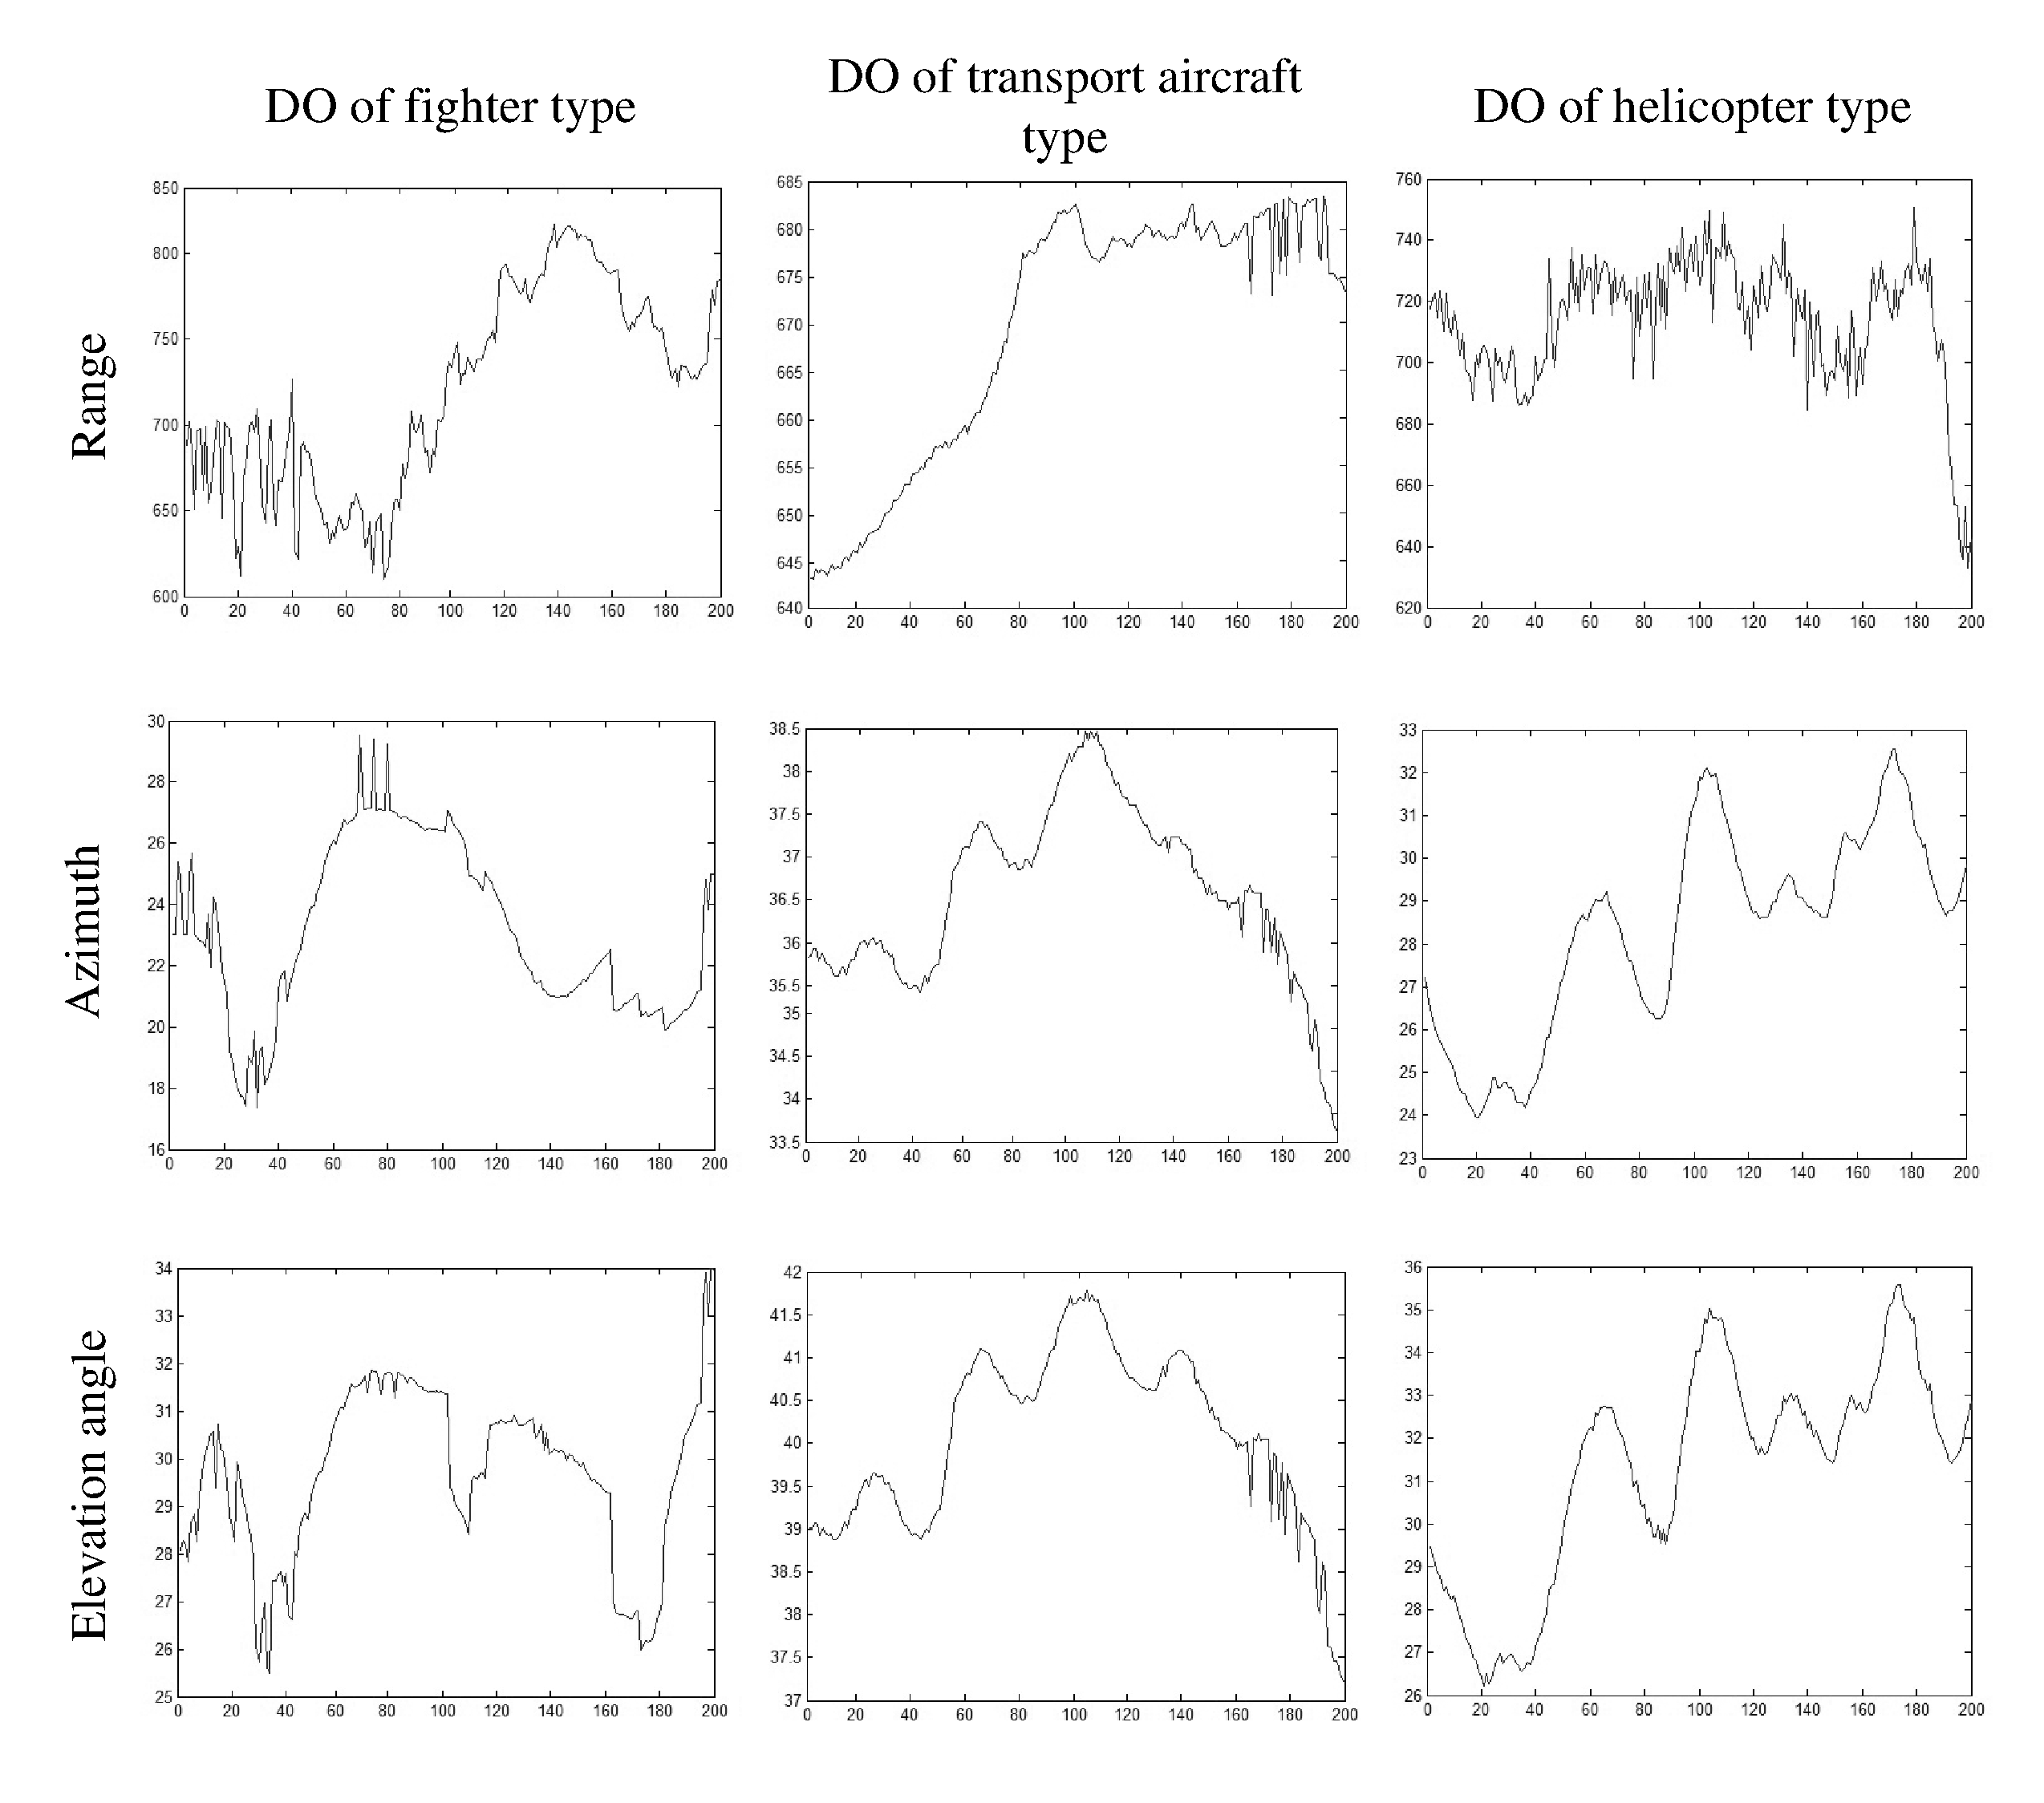
\includegraphics[width=1.0\textwidth]{pics/fig_1_option_1.pdf}
\captionstyle{normal}\caption{The samples of DO coordinate measuring for different angles of standard flight trajectory their observations by OED. Option 1.}\label{fig:fig_1_option_1}
\end{figure}

\begin{figure}[h]
\setcaptionmargin{5mm}
\onelinecaptionstrue
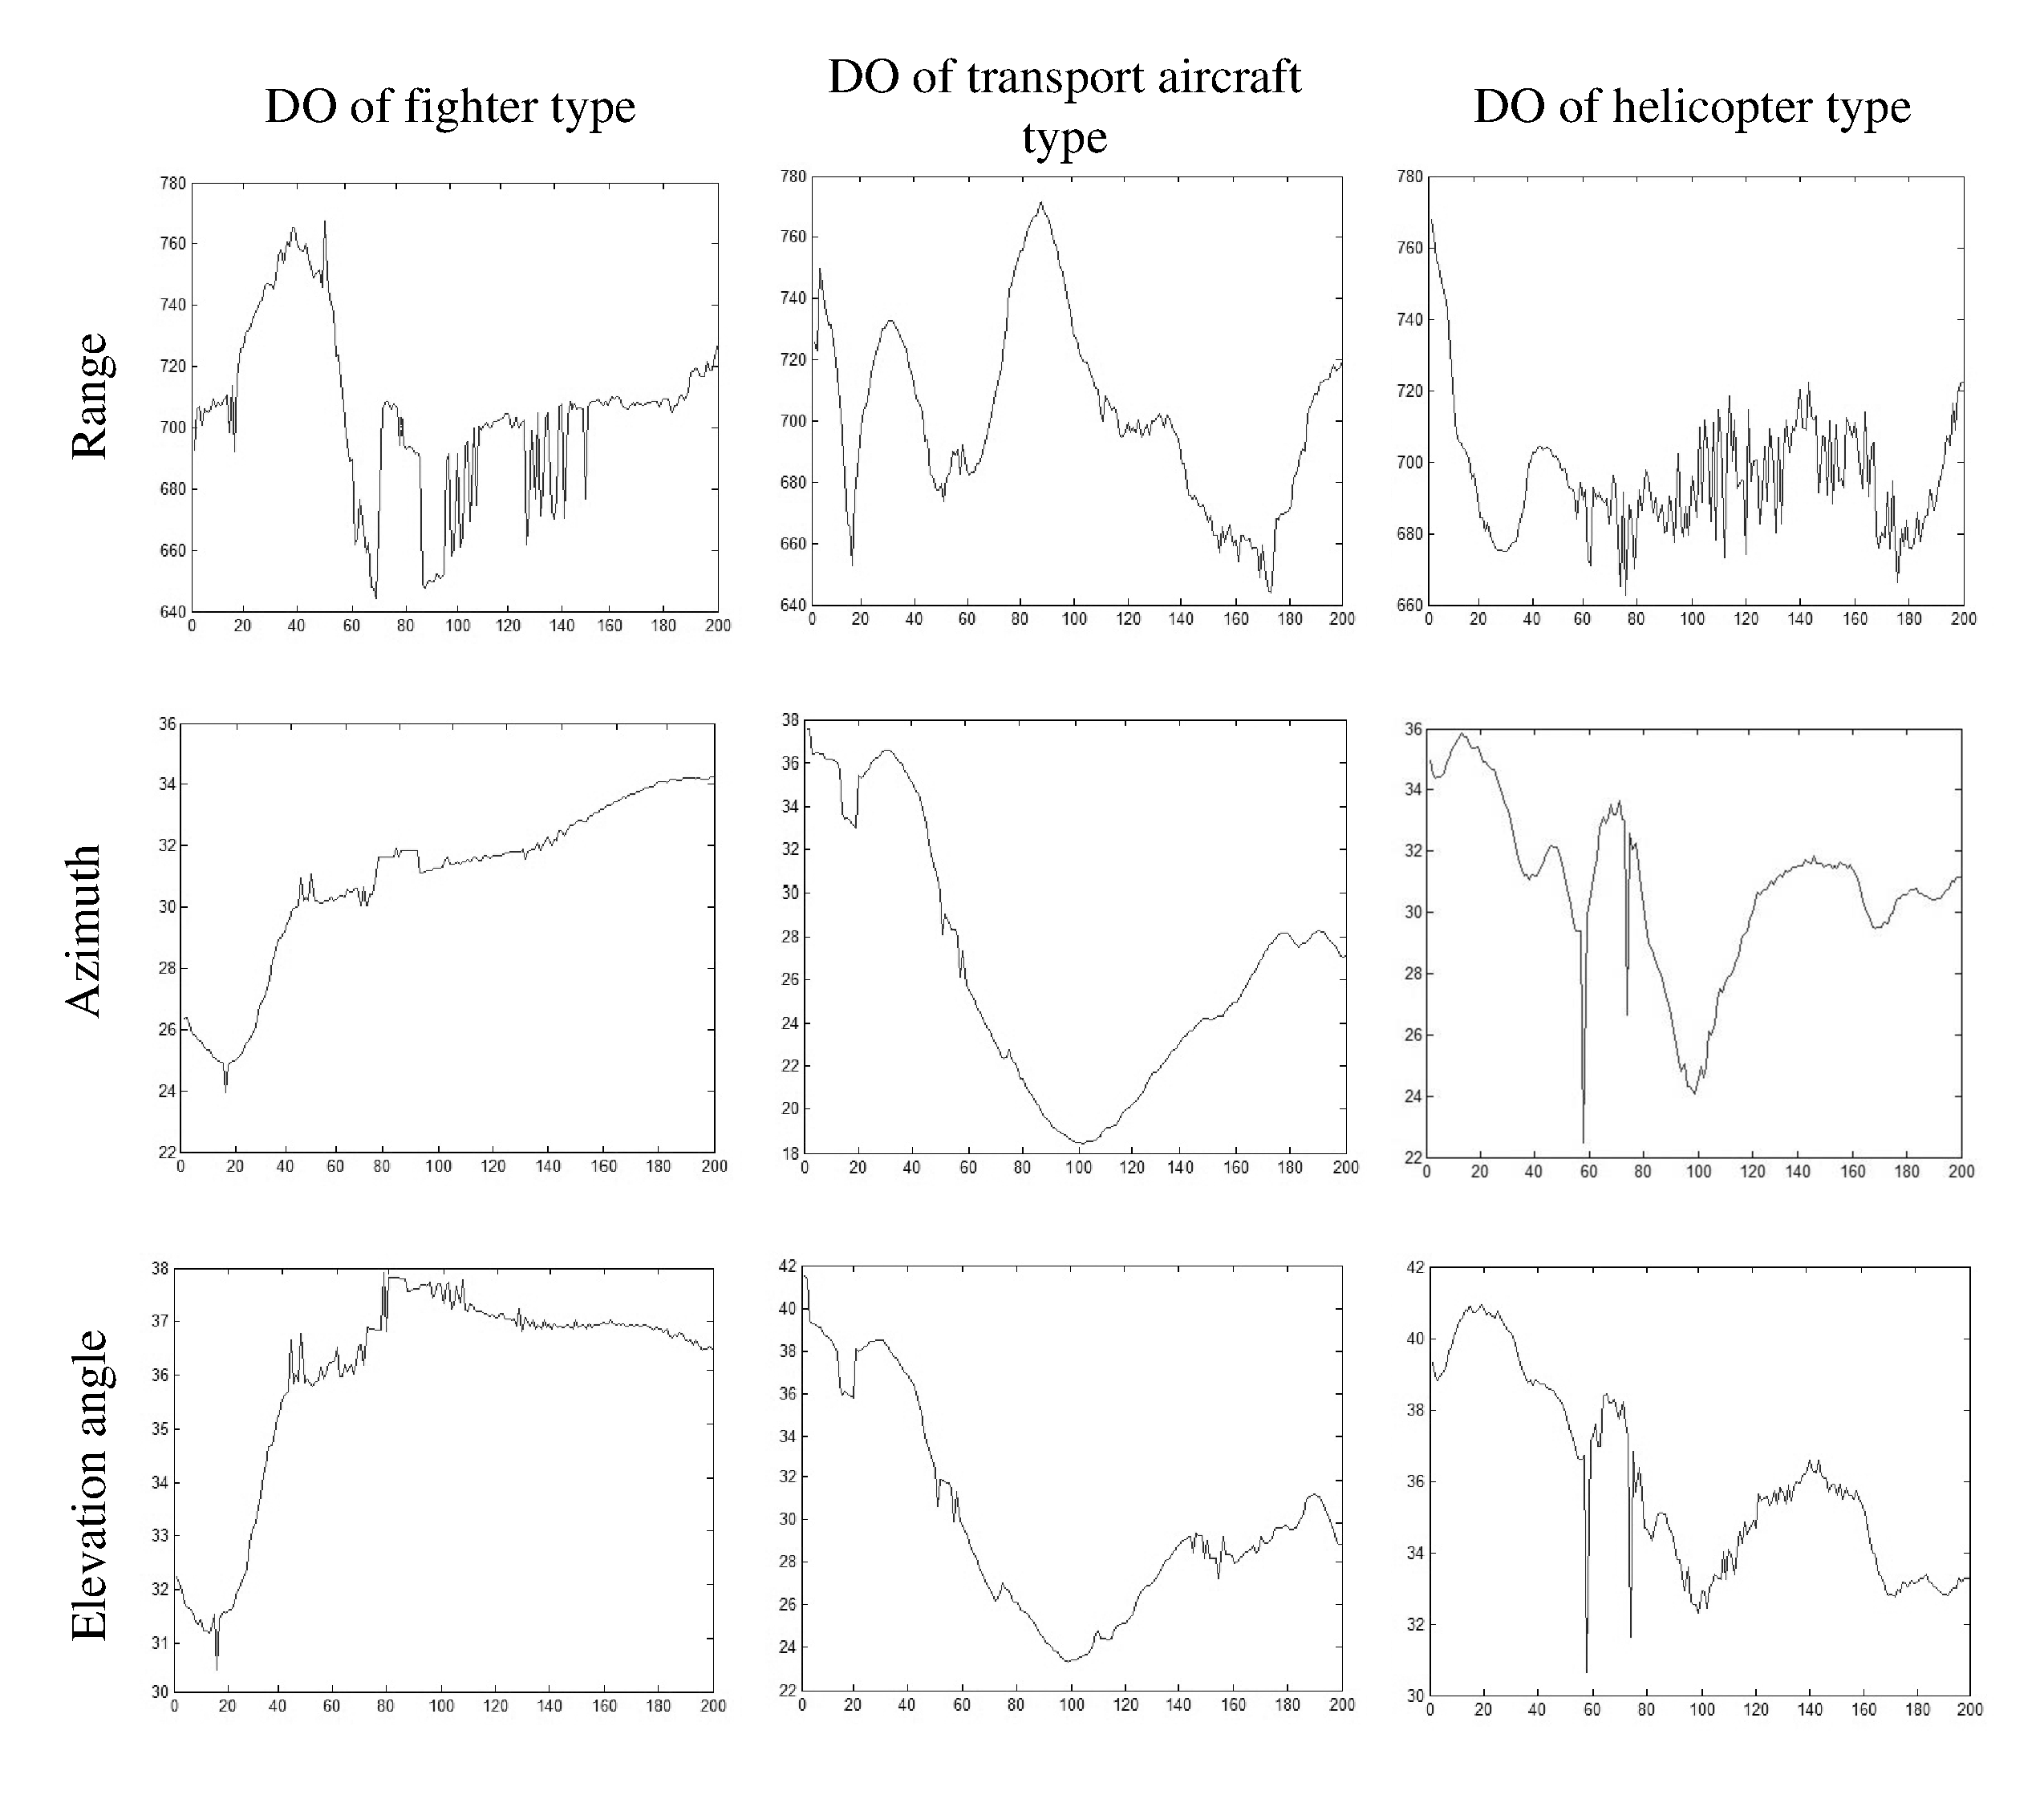
\includegraphics[width=1.0\textwidth]{pics/fig_1_option_2.pdf}
\captionstyle{normal}\caption{The samples of DO coordinate measuring for different angles of standard flight trajectory their observations by OED. Option 2.}\label{fig:fig_1_option_2}
\end{figure}

\begin{figure}[h]
\setcaptionmargin{5mm}
\onelinecaptionstrue
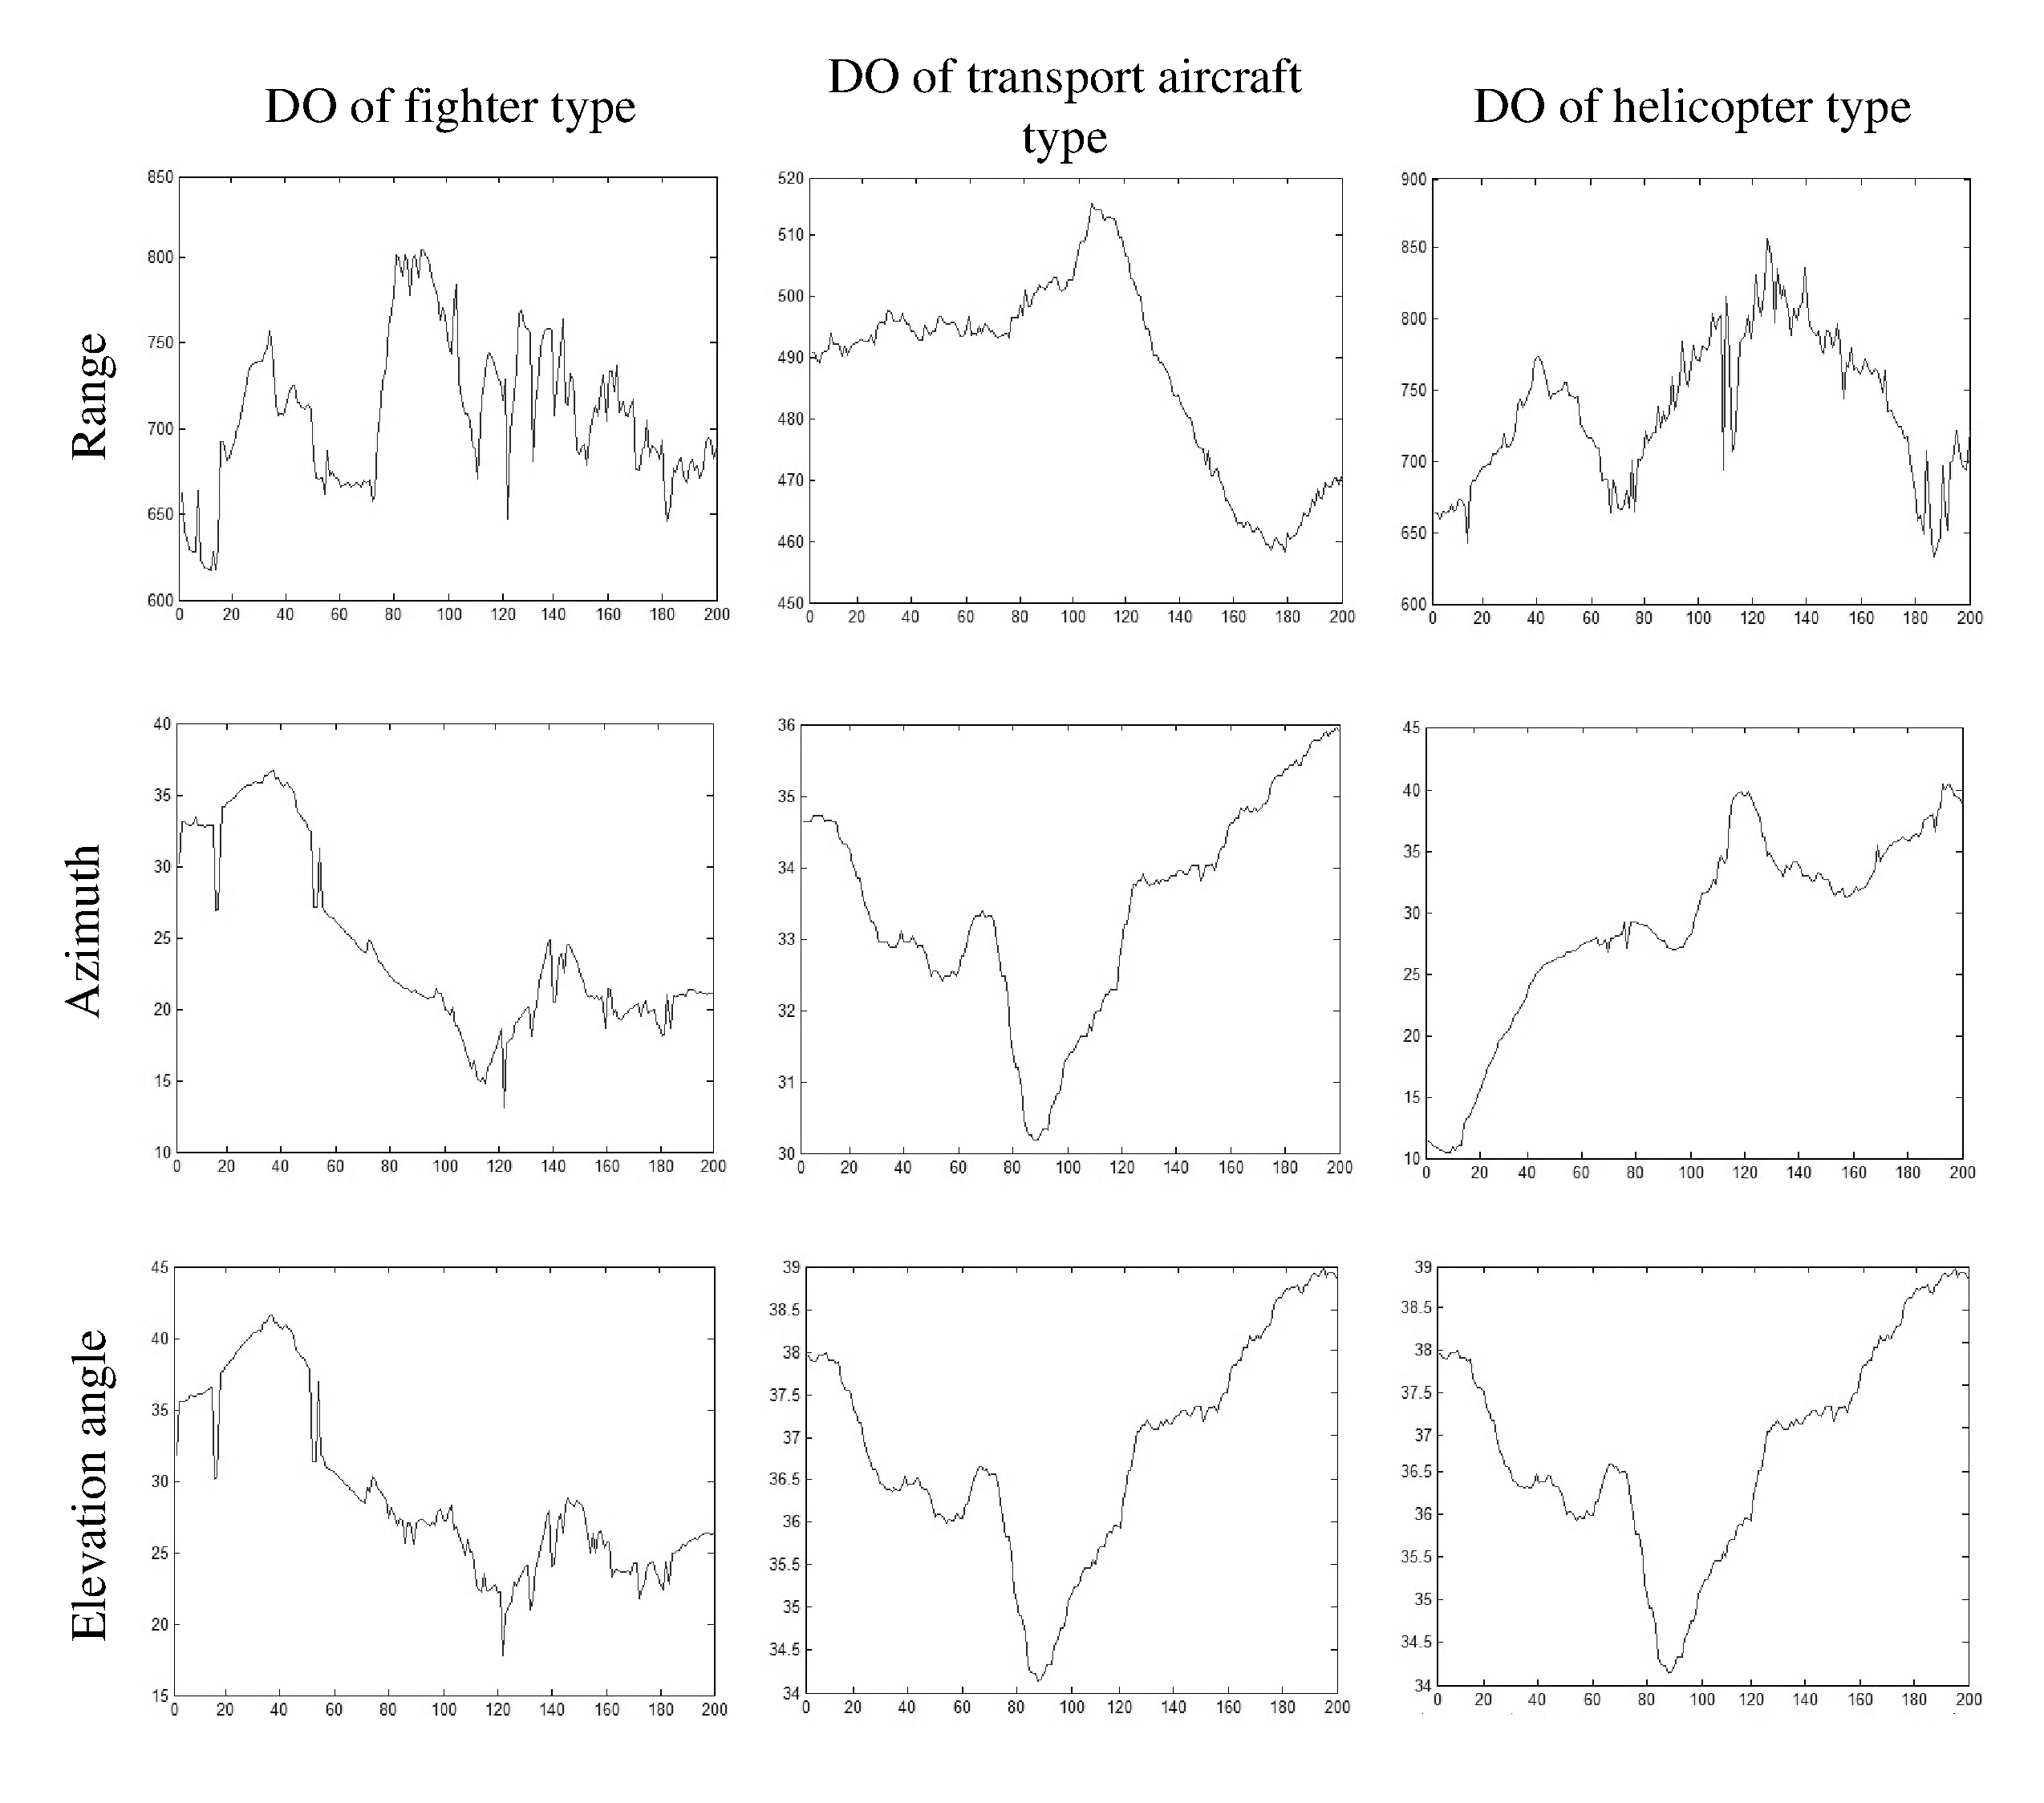
\includegraphics[width=1.0\textwidth]{pics/fig_1_option_3.pdf}
\captionstyle{normal}\caption{The samples of DO coordinate measuring for different angles of standard flight trajectory their observations by OED. Option 3.}\label{fig:fig_1_option_3}
\end{figure}
